\infolevone{
\chapter[Trigger Hardware and Software]{Trigger Hardware and Software}
\footnote{Authors: S. Boiarinov \email{boiarino@jlab.org}}

\section{Overview}
Here we give a brief overview of the 
hall A trigger, including its hardware arrangement,
the logic of the trigger, and the usage
of the software control.
Diagrams of the hardware layout are shown in
accompanying figures.

The trigger design is quite flexible and it
is relatively easy to add detectors to define
new trigger types or to modify existing ones,
so long as the detector is fast enough.
The trigger supervisor also allows for the
possibility of 2nd level triggers which could
be used for a later decision.
}

\infolevone{

\section{Components}
The trigger schematics is shown in Fig. \ref{fig:strig}.

\begin{figure}
\begin{center}
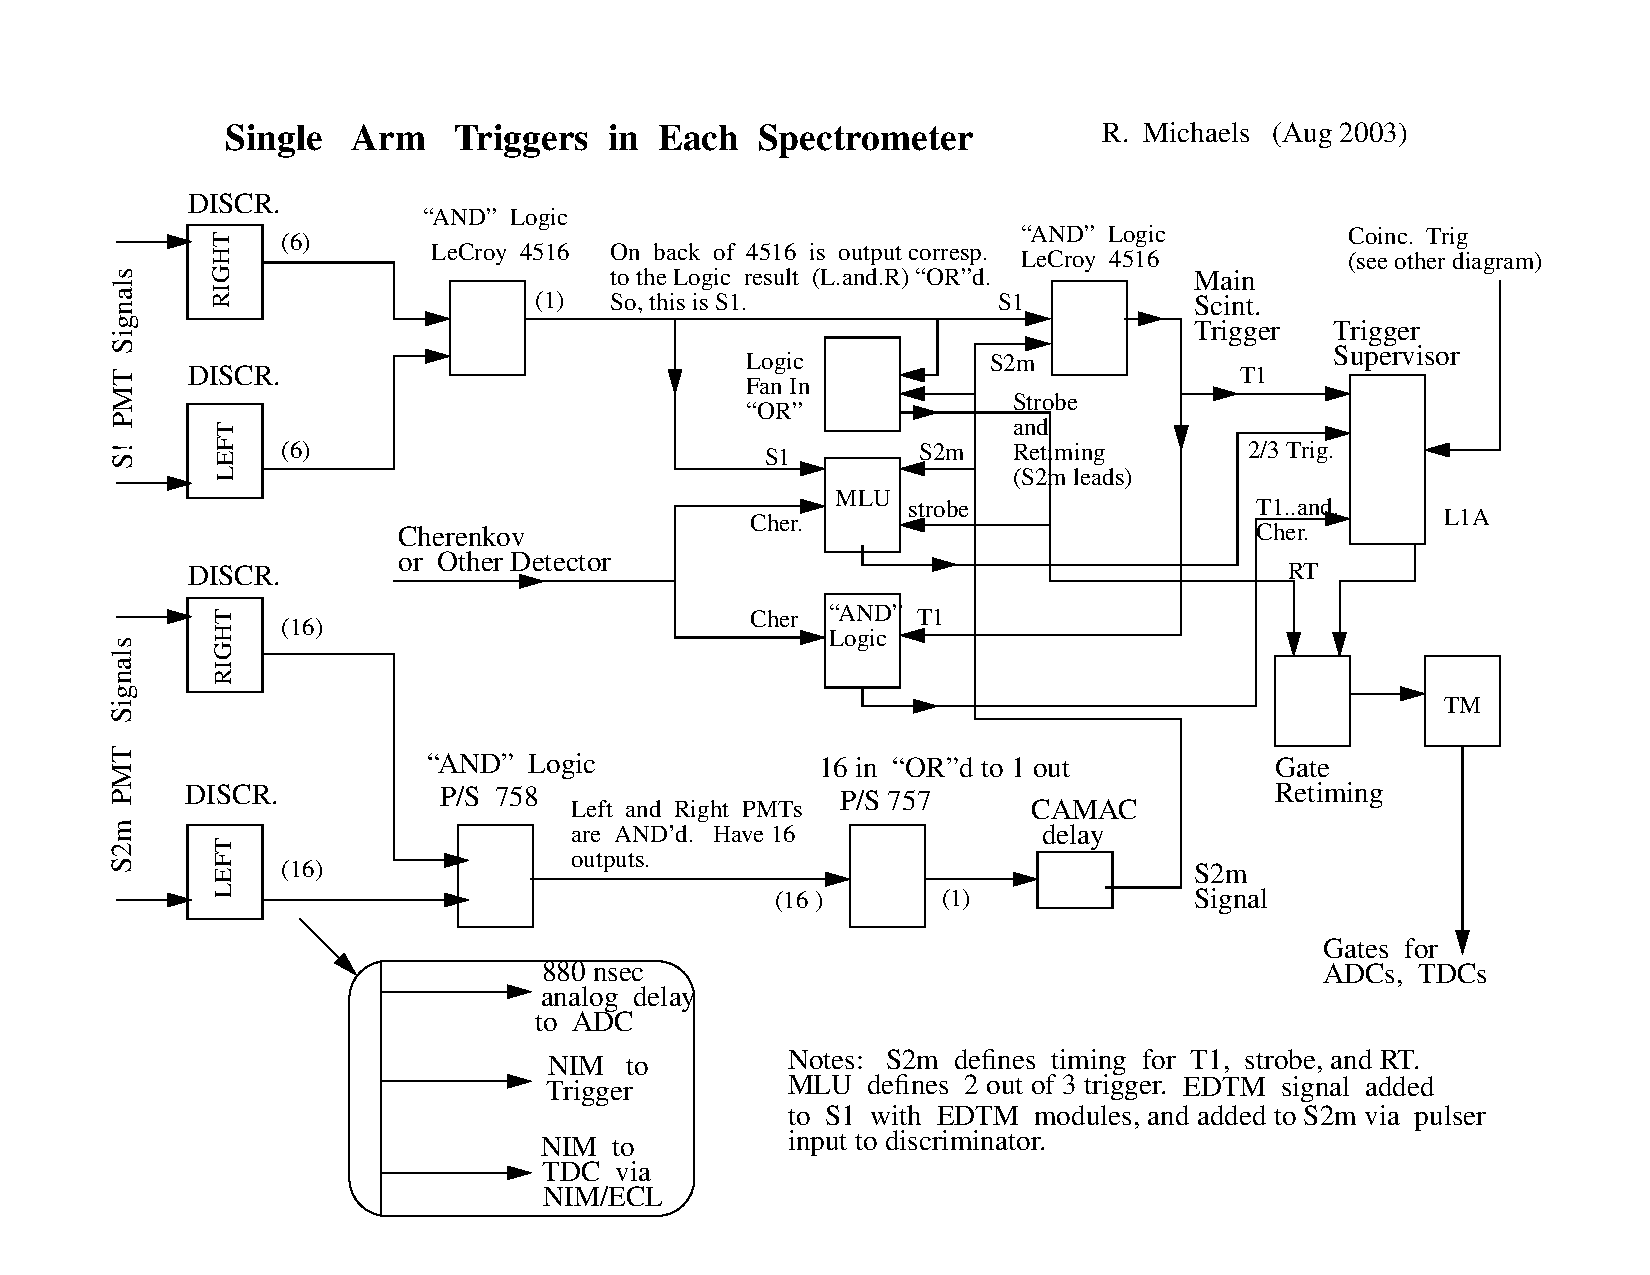
\includegraphics[angle=0,width=15cm,clip]{strig}
{\linespread{1.}
\caption[Data Acquisition: Trigger]{Trigger Circuit.}
\label{fig:strig}}
\end{center}
\end{figure}
} %infolev

\infolevtwo{
Here we describe the software control
of the  modules involved in the trigger.

Here are the instructions to download the trigger.

The user should look for suspicious 
error messages in the window from which trigsetup was 
launched, e.g. to check if connection to the crate is ok. 

If individual modules need to be modified
for test purposes etc. (e.g. to change thresholds),
one may use the expert mode.
}

\infolevone{
\begin{safetyen}{10}{15}
\subsection{Authorized  Personnel} 
\end{safetyen}
The authorized personnel is shown in table \ref{tab:trig:personnel}.
\begin{namestab}{tab:trig:personnel}{Trigger: authorized personnel}{%
      Trigger: authorized personnel.}
  \SergeiBoiarinov{\em Contact}
  \ValeryKubarovsky{}
\end{namestab}
}
